\documentclass[a4paper,12pt,oneside]{book}

%-------------------------------Start of the Preable------------------------------------------------
\usepackage[english]{babel}
\usepackage{blindtext}
%packagr for hyperlinks
\usepackage{hyperref}
\hypersetup{
    colorlinks=true,
    linkcolor=blue,
    filecolor=magenta,
    urlcolor=cyan,
}

\urlstyle{same}
%use of package fancy header
\usepackage{fancyhdr}
\setlength\headheight{26pt}
\fancyhf{}
%\rhead{
\includegraphics[width=1cm]{logo}}
\lhead{\rightmark}
\rhead{
\includegraphics[width=1cm]{logo}}
\fancyfoot[RE, RO]{\thepage}
\fancyfoot[CE,CO]{\href{http://www.e-yantra.org}{www.e-yantra.org}}

\pagestyle{fancy}

%use of package for section title formatting
\usepackage{titlesec}
\titleformat{\chapter}
  {\Large\bfseries} % format
  {}                % label
  {0pt}             % sep
  {\huge}           % before-code

%use of package tcolorbox for colorful textbox
\usepackage[most]{tcolorbox}
\tcbset{colback=cyan!5!white,colframe=cyan!75!black,halign title = flush center}

\newtcolorbox{mybox}[1]{colback=cyan!5!white,
colframe=cyan!75!black,fonttitle=\bfseries,
title=\textbf{\Large{#1}}}

%use of package marginnote for notes in margin
\usepackage{marginnote}

%use of packgage watermark for pages
%\usepackage{draftwatermark}
%\SetWatermarkText{
\includegraphics{logo}}
\usepackage[scale=2,opacity=0.1,angle=0]{background}
\backgroundsetup{
contents={
\includegraphics{logo}}
}

%use of newcommand for keywords color
\usepackage{xcolor}
\newcommand{\keyword}[1]{\textcolor{red}{\textbf{#1}}}

%package for inserting pictures
\usepackage{graphicx}

%package for highlighting
\usepackage{color,soul}

%new command for table
\newcommand{\head}[1]{\textnormal{\textbf{#1}}}


%----------------------End of the Preamble---------------------------------------


\begin{document}

%---------------------Title Page------------------------------------------------
\begin{titlepage}
\raggedright
{\Large eYSIP2016\\[1cm]}
{\Huge\scshape Tiva Manual\\[.1in]}
\vfill
\begin{flushright}
{\large Amanpreet Singh \\}
{\large Amit Raushan \\}
{\large Shubham Gupta \\}
{\large Duration of Internship: $ 10/06/2016-24/07/2016 $ \\}
\end{flushright}

{\itshape 2016, e-Yantra Publication}

\end{titlepage}

\tableofcontents

%------------------------------------------------------------------------

\chapter[Tiva Manual]{Tiva Manual}
\section{Abstract}

This manual is related to use of \textbf{Tiva� C Series TM4C123G LaunchPad Evaluation Board} to make a robot which includes two DC geared motor, a pair of wheels, 3 channel white line sensor, 1 Sharp sensor, buzzer \& one 16x2 LCD display.\par
In case we need to transfer data from the robot to laptop/PC we can interface a XBee module with Tiva board. We can use this robot to get familiar with Tiva board and further it can be developed to do real world tasks. For example, the basic  robot developed here can be programmed to work as white line sensing robot or as wall follower robot.
\newpage
\section{Board Overview}

\begin{figure}[h]
\centering
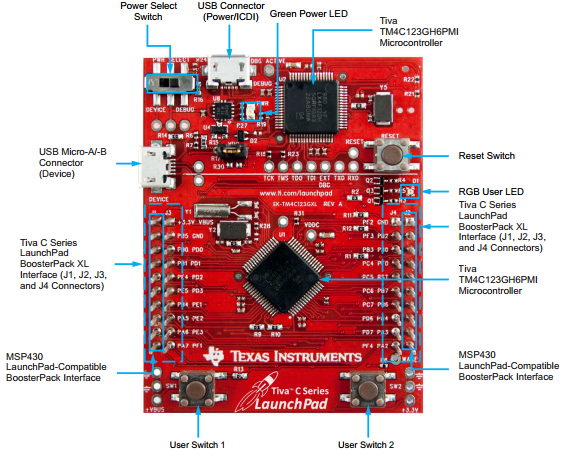
\includegraphics[scale=1]{board}
\caption{Tiva C Series TM4C123G LaunchPad Evaluation Board}
\end{figure}
This launchpad contains TM4C123GH6PM as microcontroller.\\
The TM4C123GH6PM is a 32-bit ARM Cortex-M4-based microcontroller with 256-kB Flash memory, 32\-kB SRAM and 80-MHz operation; USB host, device and OTG connectivity; a Hibernation module and PWM; and many other peripherals.
\newpage
\subsection{Kit Contents [Source: Tiva� C Series TM4C123G LaunchPad User's Guide]}
The Tiva C Series TM4C123G LaunchPad Evaluation Kit contains the following items:
\begin{itemize}
    \item Tiva C Series LaunchPad Evaluation Board (EK-TM4C123GXL).
    \item On-board In-Circuit Debug Interface (ICDI)
    \item USB micro-B plug to USB-A plug cable.

\end{itemize}
\subsection{Features [Source: Source: Tiva� C Series TM4C123G LaunchPad User's Guide]}
Tiva C Series LaunchPad includes the following features:
\begin{itemize}
    \item Tiva TM4C123GH6PMI microcontroller.
    \item Motion control PWM.
    \item USB micro-A and micro-B connector for USB device, host, and on-the-go (OTG) connectivity.
    \item RGB user LED.
    \item Two user switches (application/wake)
    \item Available I/O brought out to headers on a 0.1-in (2.54-mm) grid.
    \item On-board ICDI.
    \item Switch-selectable power sources:
    \begin{itemize}
      \item  ICDI
       \item USB device
\end{itemize}
\item Reset switch
\item Preloaded RGB quickstart application
\item Supported by TivaWare for C Series software including the USB library and the peripheral driver library
\end{itemize}
\newpage
\section{Hardware Parts Used}
\begin{enumerate}
 \item  Tiva C Series TM4C123G LaunchPad Evaluation Board.

 \href{http://www.ti.com.cn/cn/lit/ds/symlink/tm4c123gh6pm.pdf}{ Datasheet}\\
  \href{http://www.ti.com/lit/ug/spmu298a/spmu298a.pdff}{ Pheripheral Driver Library}\\
  \href{http://www.mouser.com/ds/2/405/spmu296-242111.pdf}{User's Guide}
  \begin{figure}[h]
        \centering
        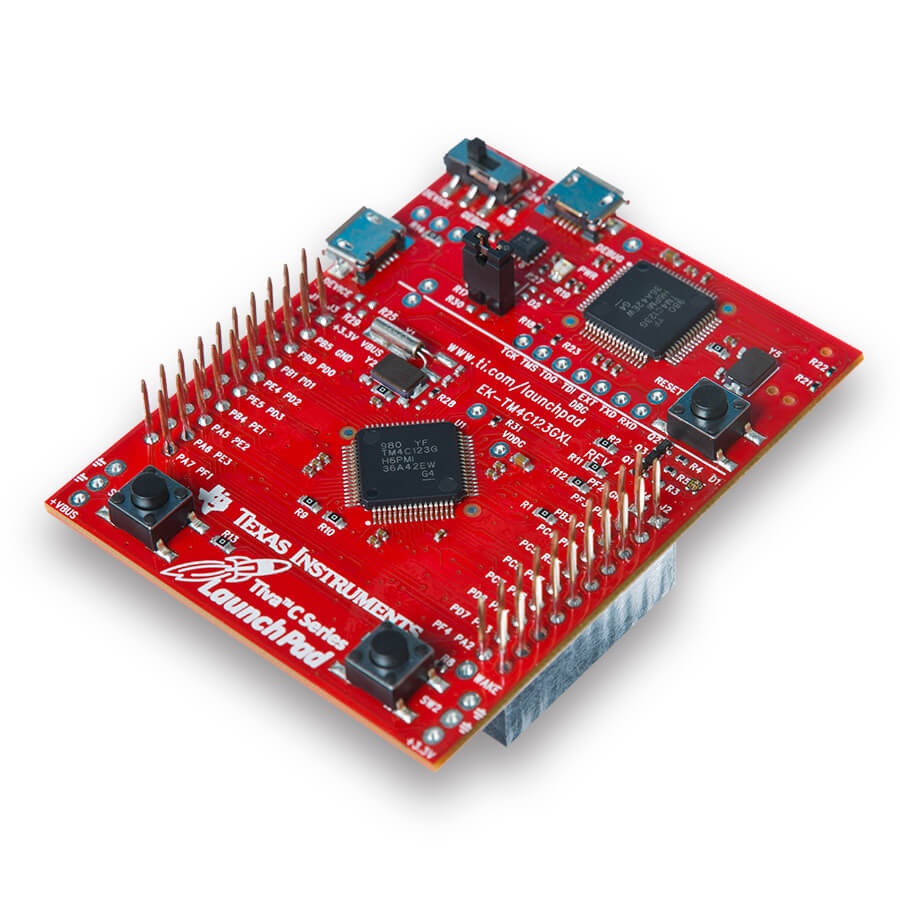
\includegraphics[scale=0.2]{tiva}
        \caption{Tiva C Series TM4C123G LaunchPad}
      \end{figure}


   \item 2x DG02S Mini DC Geared Motor.\\
   \href{http://cdn.sparkfun.com/datasheets/Robotics/DG02S.pdf}{ Datasheet}
   \begin{figure}[!ht]
        \centering
        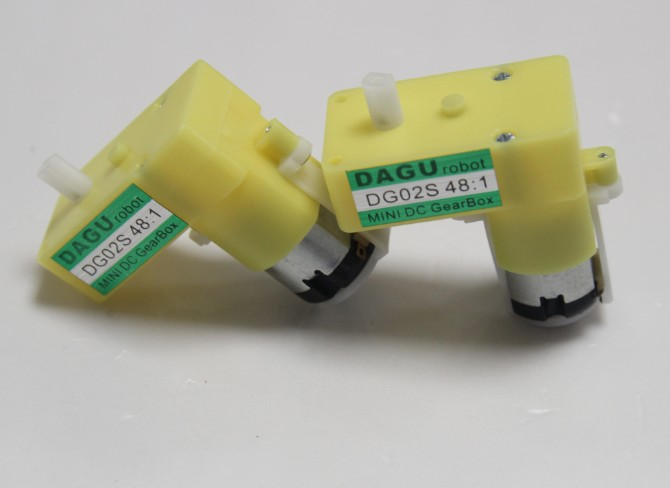
\includegraphics[scale=0.3]{motor}
        \caption{DC Geared Motor}
      \end{figure}
\newpage
    \item 2x Wheel - 65mm in Diameter
    \begin{figure}[h]
        \centering
        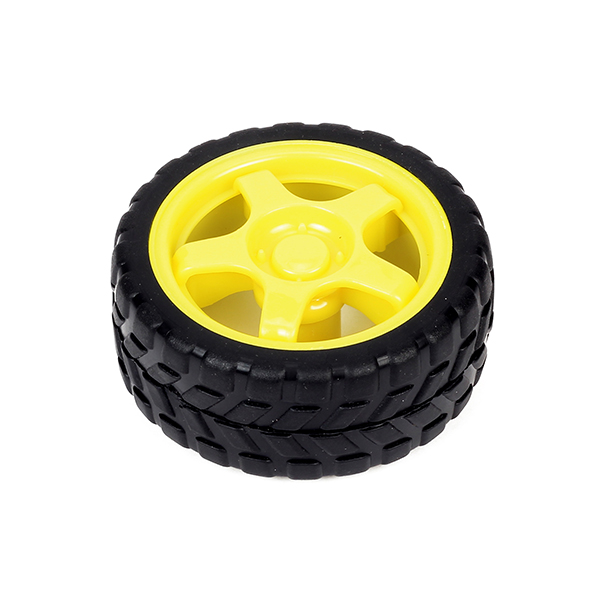
\includegraphics[scale=0.22]{wheel}
        \caption{Wheel}
      \end{figure}
    \item L293D - Motor Driver.\\
    \href{http://www.engineersgarage.com/sites/default/files/L293D.pdf}{ Datasheet}\par
   \begin{figure}[!ht]
        \centering
        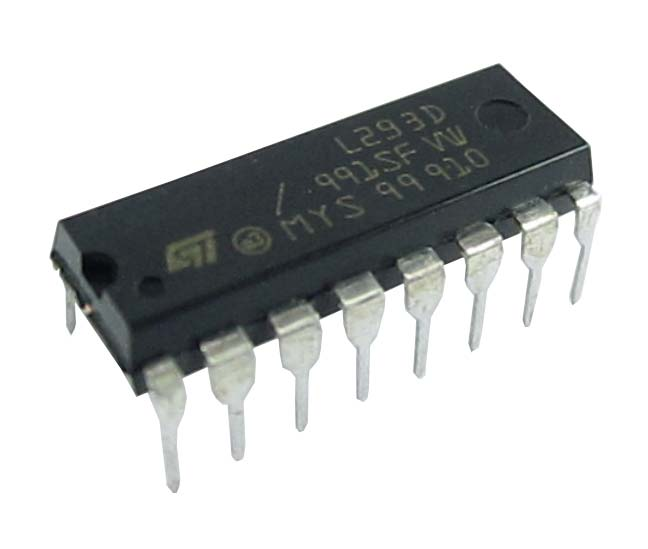
\includegraphics[scale=0.2]{l293d}
        \caption{Motor Driver IC}
      \end{figure}
    \item 16x2 LCD.\\
    \href{http://www.engineersgarage.com/sites/default/files/LCD\%2016x2.pdf}{ Datasheet}\par
   \begin{figure}[!ht]
        \centering
        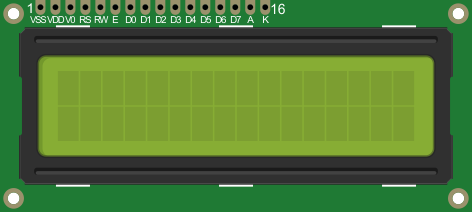
\includegraphics[scale=0.85]{lcd}
        \caption{LCD 16x2 Display}
      \end{figure}
      \newpage
    \item White Line Sensor Module.\\
    \href{http://www.nex-robotics.com/images/downloads/3\%20channel\%20line\%20sensor.pdf}{ Manual}\par
   \begin{figure}[!ht]
        \centering
        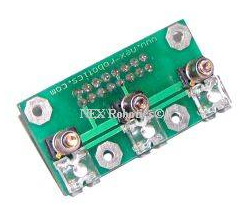
\includegraphics[scale=0.85]{whiteline}
        \caption{3 Channel White Line Sensors}
      \end{figure}
    \item Sharp 0A41SK Sensor.\\
    \href{http://www.sharp-world.com/products/device/lineup/data/pdf/datasheet/gp2y0a41sk_e.pdf}{ Datasheet}\par
   \begin{figure}[!ht]
        \centering
        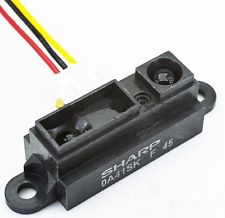
\includegraphics[scale=0.7]{sharp}
        \caption{Sharp Sensor}
      \end{figure}
    \item Caster Wheel.
    \begin{figure}[!ht]
        \centering
        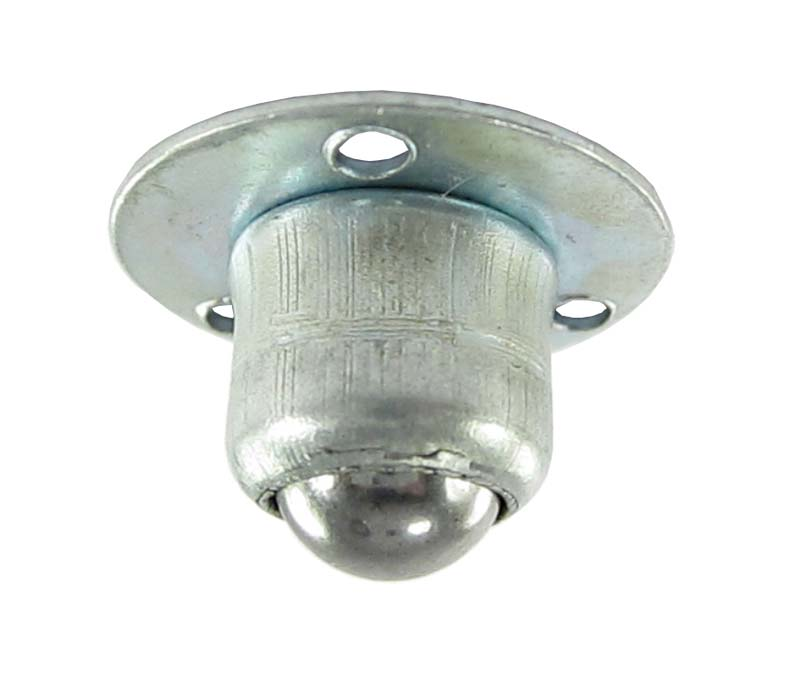
\includegraphics[scale=0.15]{caster}
        \caption{Caster Wheel}
      \end{figure}
      \newpage

    \item LM3237 - Voltage Regulator.\\
    \href{http://pdf.datasheetarchive.com/indexerfiles/Datasheet-044/DSA0017815.pdf}{ Datasheet}\par
   \begin{figure}[!ht]
        \centering
        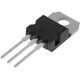
\includegraphics[scale=0.9]{lm}
        \caption{LM3237}
      \end{figure}
    \item Heat Sink.
    \begin{figure}[!ht]
        \centering
        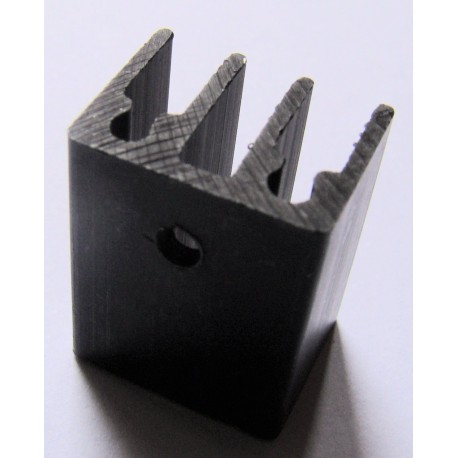
\includegraphics[scale=0.25]{heat}
        \caption{Heat Sink}
      \end{figure}
    \item 10 uF Electrolyte Capacitor.
    \begin{figure}[!ht]
        \centering
        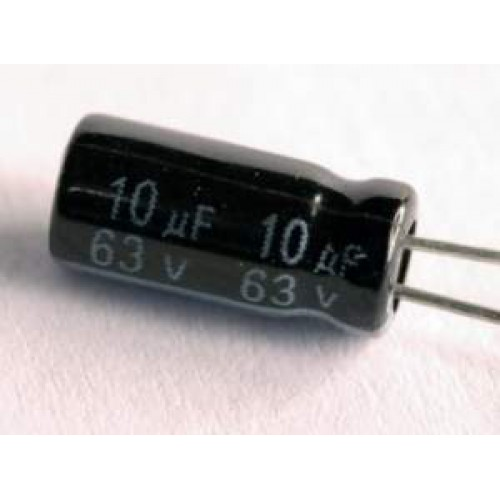
\includegraphics[scale=0.35]{cap}
        \caption{Capacitor}
      \end{figure}
      \newpage
    \item Multi-purpose PCB board. \\
    \begin{figure}[!h]
        \centering
        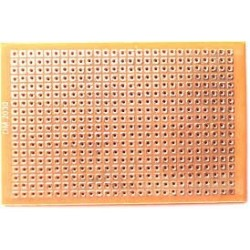
\includegraphics[scale=0.6]{pcb}
        \caption{PCB Board}
      \end{figure}
    \item 12V Rechargeable Battery.
    \begin{figure}[!h]
        \centering
        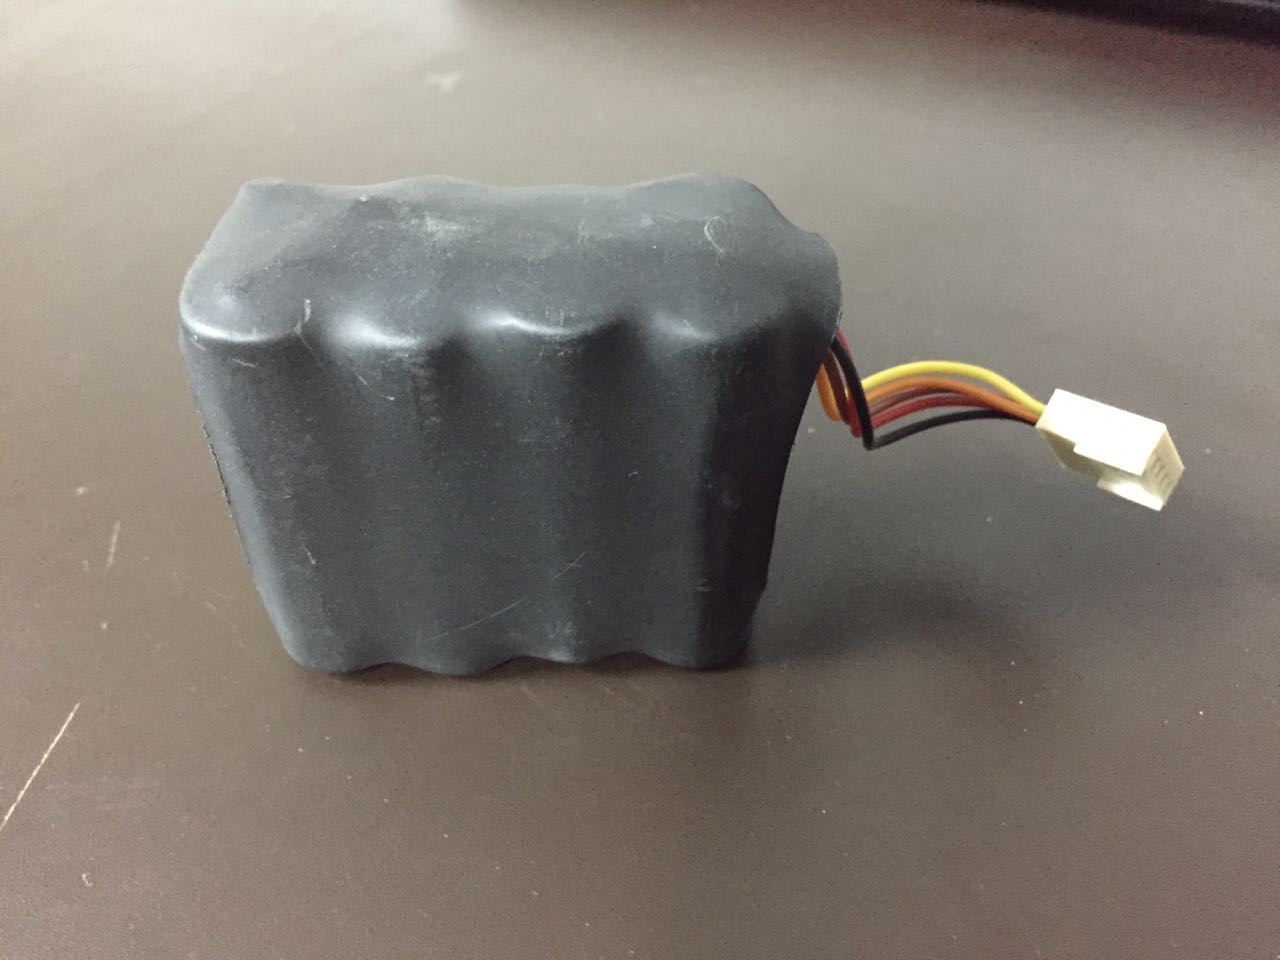
\includegraphics[scale=0.12]{battery}
        \caption{12V Rechargeable Battery}
      \end{figure}
      \newpage
    \item 20 Pin Planar Cable.
    \begin{figure}[!h]
        \centering
        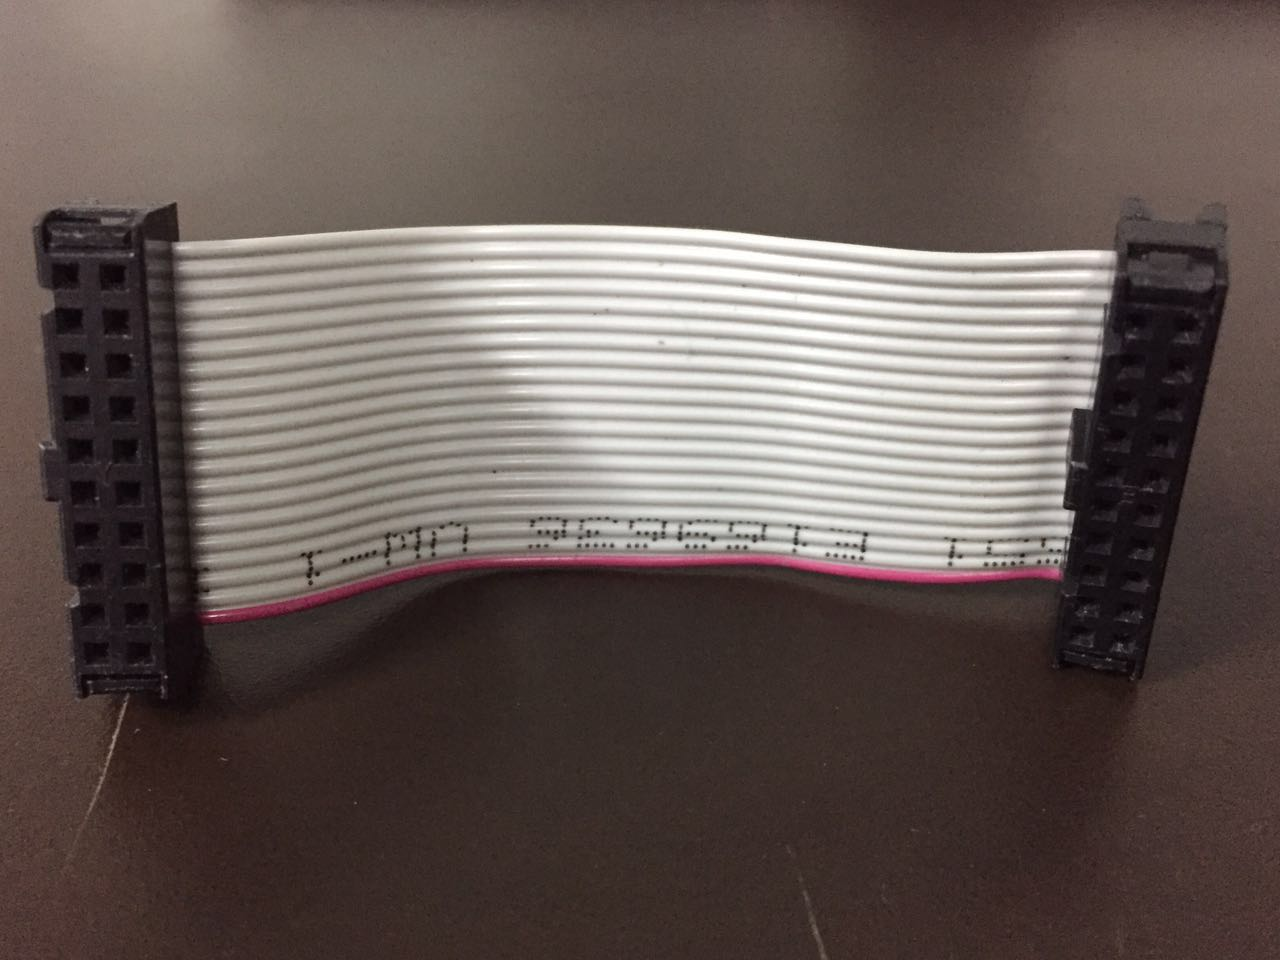
\includegraphics[scale=0.1]{wire}
        \caption{20 Pin Connector Wire}
      \end{figure}
    \item Female Bug Strip.
    \\
    \begin{figure}[!h]
        \centering
        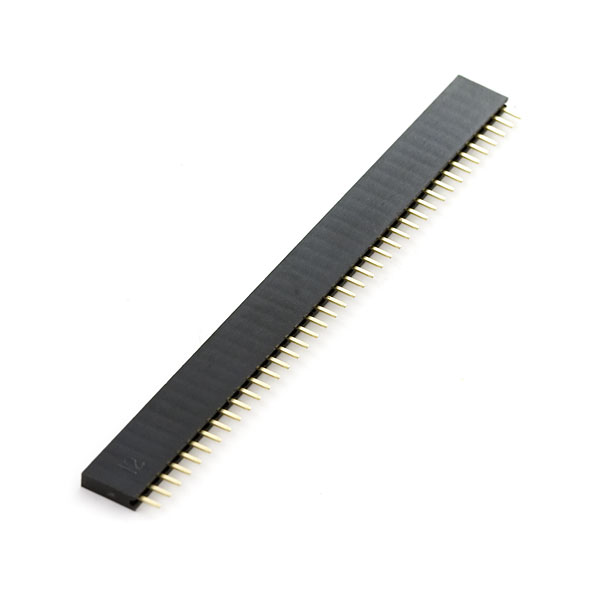
\includegraphics[scale=0.2]{fmbug}
        \caption{Female Bug Strip}
      \end{figure}
    \item Male Bug Strip.
    \begin{figure}[!h]
        \centering
        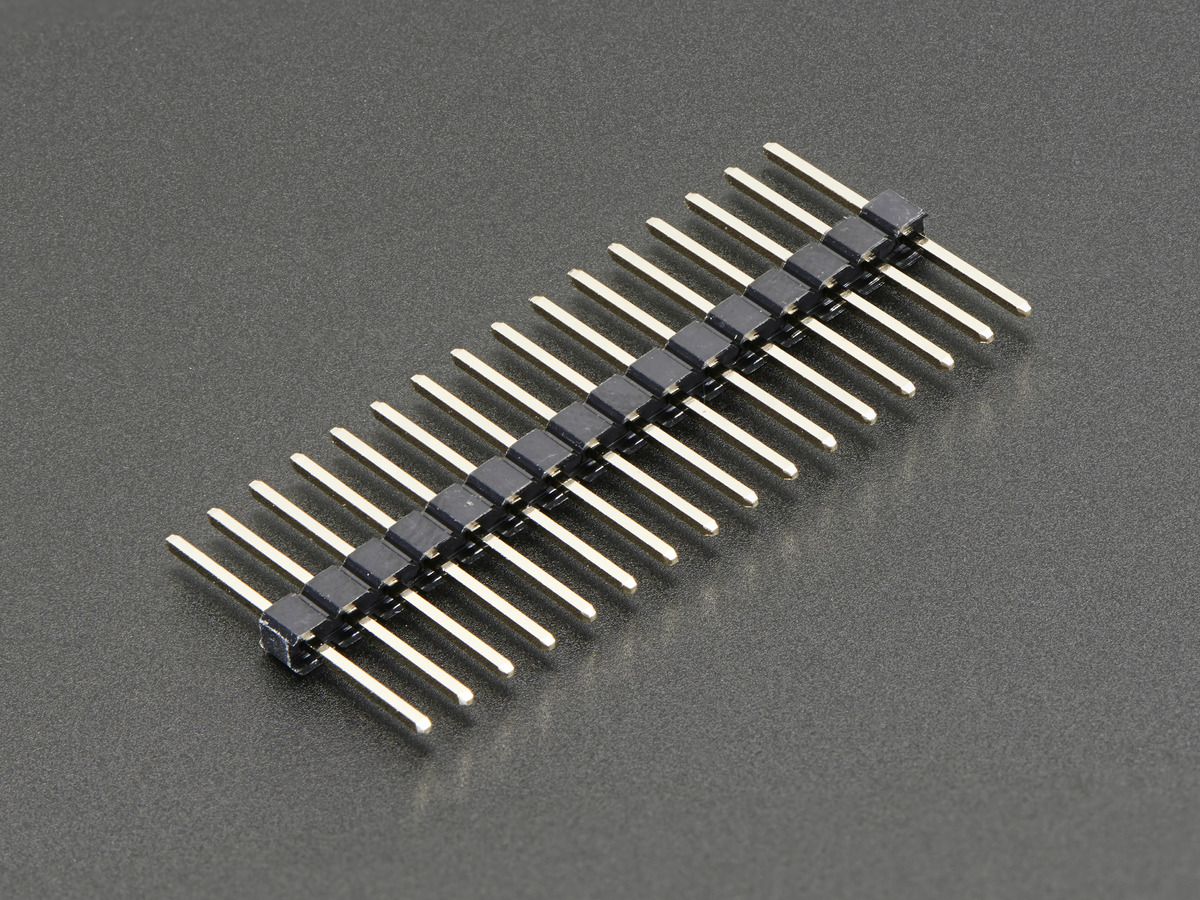
\includegraphics[scale=0.12]{mbug}
        \caption{Male Bug Strip}
      \end{figure}
      \newpage
    \item Male to Female Jumper Wires.
    \begin{figure}[!h]
        \centering
        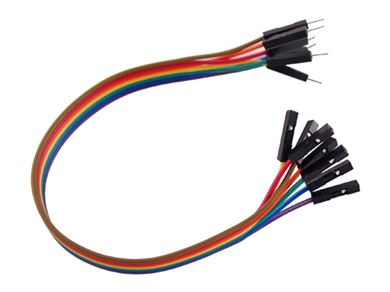
\includegraphics[scale=0.45]{jumper}
        \caption{Jumper Wires}
      \end{figure}\\
    \item Plastic Chassis.\\
     \par
    \begin{figure}[!h]
        \centering
        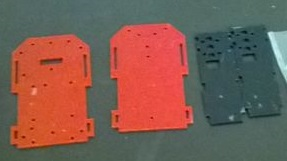
\includegraphics[scale=0.75]{chasis}
        \caption{Chassis}
      \end{figure}
    \item XBee Module.
     \begin{figure}[!h]
        \centering
        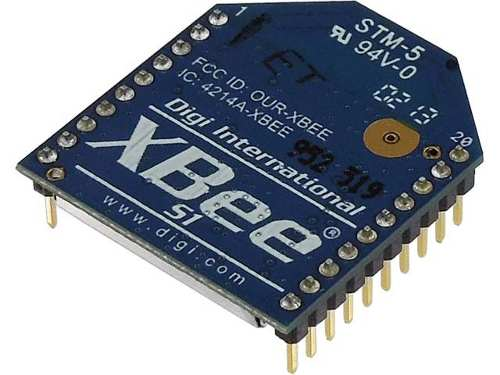
\includegraphics[scale=0.2]{xbee.jpg}
        \caption{XBee Module}
      \end{figure}
        \end{enumerate}
 \newpage
 \section{Interfacing of Hardwares }
\subsection{Tiva Robot}

\begin{figure}[h]
	\centering
	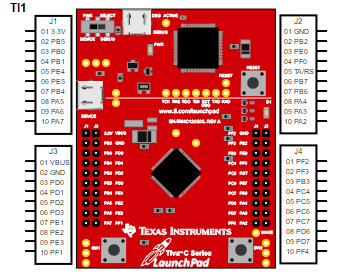
\includegraphics[scale=1]{Tiva_pin}
	\caption{Tiva Board Pin Location}
\end{figure}

Connections of PORT pins of Tiva board with different components:\\
\begin {enumerate}
\item Interfacing of White Line Sensor
\begin{center}
	\begin{figure}[h]
		\centering
		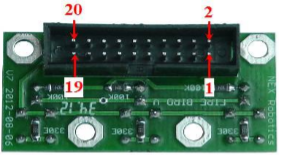
\includegraphics[scale=1]{whiteline_pin}
		\caption{Pin Configuration of White Line Sensor}
	\end{figure}
	
	\begin{tabular}{| c | c |}
		
		\hline
		\textbf{Tiva Port Pins} & \textbf{Sensors Pin}\\
		
		\hline
		PE1 & 1\\
		\hline
		PE2 & 3\\
		\hline
		PE3 & 5 \\
		\hline
		VCC & 2\\
		\hline
		VCC & 4 \\
		\hline
		VCC & 6 \\
		\hline
		GND & 15\\
		\hline
		GND & 16\\
		\hline
		GND & 17\\
		\hline
		VCC & 19 \\
		\hline
	\end{tabular}
\end{center}


\item Interfacing of XBee Module\\
\begin{figure}[h]
	\centering
	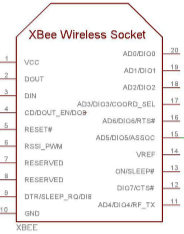
\includegraphics[scale=1]{XBee}
	\caption{Pin Configuration of XBee Socket}
\end{figure}
\begin{center}
	\begin{tabular}{| c | c |}
		\hline
		\textbf{Tiva Port Pins} & \textbf{XBee Pins}\\
		\hline
		PC4 & DOUT\\
		\hline
		PC5 & DIN\\
		\hline
		GND & GND\\
		\hline
		VCC & VCC \\
		\hline
	\end{tabular}
\end{center}
\newpage
\item Interfacing of Sharp Sensor\\
\begin{center}
	\begin{tabular}{| c | c |}
		\hline
		\textbf{Tiva Port Pins} & \textbf{Sensor Pins}\\
		\hline
		PE0 & SIGNAL\\
		\hline
		GND & GND\\
		\hline
		VCC & VCC \\
		\hline
	\end{tabular}
\end{center}
\item Interfacing of Motor Driver IC\\
\begin{figure}[h]
	\centering
	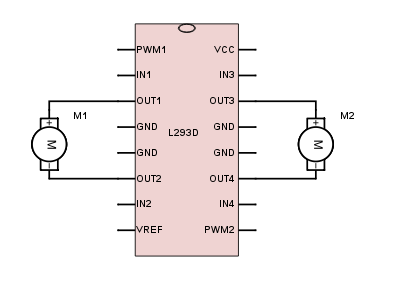
\includegraphics[scale=1]{MOTOR_DRIVER}
	\caption{Pin Configuration of Motor Driver IC}
\end{figure}
\begin{center}
	\begin{tabular}{| c | c |}
		\hline
		\textbf{Tiva Port Pins} & \textbf{L293D Pins}\\
		\hline
		PE4 & PWM1\\
		\hline
		PA2 & INPUT1\\
		\hline
		PA3 & INPUT2 \\
		\hline
		GND & GND\\
		\hline
		VCC & VCC \\
		\hline
		PE5 & PWM2 \\
		\hline
		PA6 & INPUT3\\
		\hline
		PA7 & INPUT4 \\
		\hline
		VBUS & VREF \\
		\hline
	\end{tabular}
\end{center}

\item Interfacing of Buzzer
\begin{figure}[h]
	\centering
	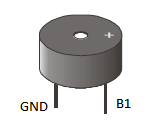
\includegraphics[scale=1]{speaker}
	\caption{Pin Configuration of Buzzer}
\end{figure}
\begin{center}
	\begin{tabular}{| c | c |}
		\hline
		\textbf{Tiva Port Pins} & \textbf{Buzzer Pins}\\
		\hline
		PF0 & B1\\
		\hline
		GND & GND\\
		\hline
	\end{tabular}
\end{center}
\newpage
\item Interfacing of LCD
\begin{figure}[h]
	\centering
	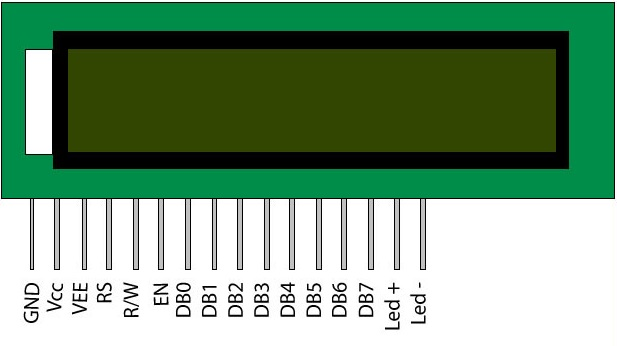
\includegraphics[scale=0.5]{lcd_pin}
	\caption{Pin Configuration of LCD Display}
\end{figure}
\begin{center}
	\begin{tabular}{| c | c |}
		\hline
		\textbf{Tiva Port Pins} & \textbf{LCD Pins}\\
		\hline
		GND & GND\\
		\hline
		VCC & Vcc\\
		\hline
		GND & VEE \\
		\hline
		PA4 & RS\\
		\hline
		PA5 & R/W \\
		\hline
		PC6 & EN \\
		\hline
		PB0 & DB0\\
		\hline
		PB1 & DB1 \\
		\hline
		PB2 & DB2\\
		\hline
		PB3 & DB3 \\
		\hline
		PB4 & DB4 \\
		\hline
		PB5 & DB5 \\
		\hline
		PB6 & DB6 \\
		\hline
		PB7 & DB7 \\
		\hline
		VCC & Led+ \\
		\hline
		GND & Led- \\
		\hline
	\end{tabular}
\end{center}
\end{enumerate}
\newpage

 \section{Block Diagram}
 \begin{figure}[!h]
        \centering
        \includegraphics[scale=0.9]{block}
        \caption{Block Diagram of Tiva Robot}
      \end{figure}
      \newpage
      \section{Voltage Regulator Circuit Diagram}
 \begin{figure}[!h]
 	\centering
 	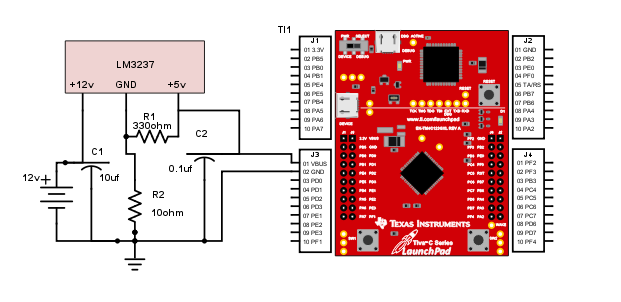
\includegraphics[scale=0.8]{LM3237}
 	\caption{Voltage Regulator Circuit Diagram}
 \end{figure}
\newpage
\subsection{Steps for Assembling Tiva Robot}
\begin{enumerate}
	\item Gather/Buy all the components to be used for building the Robot.
	\begin{figure}[h]
		\centering
		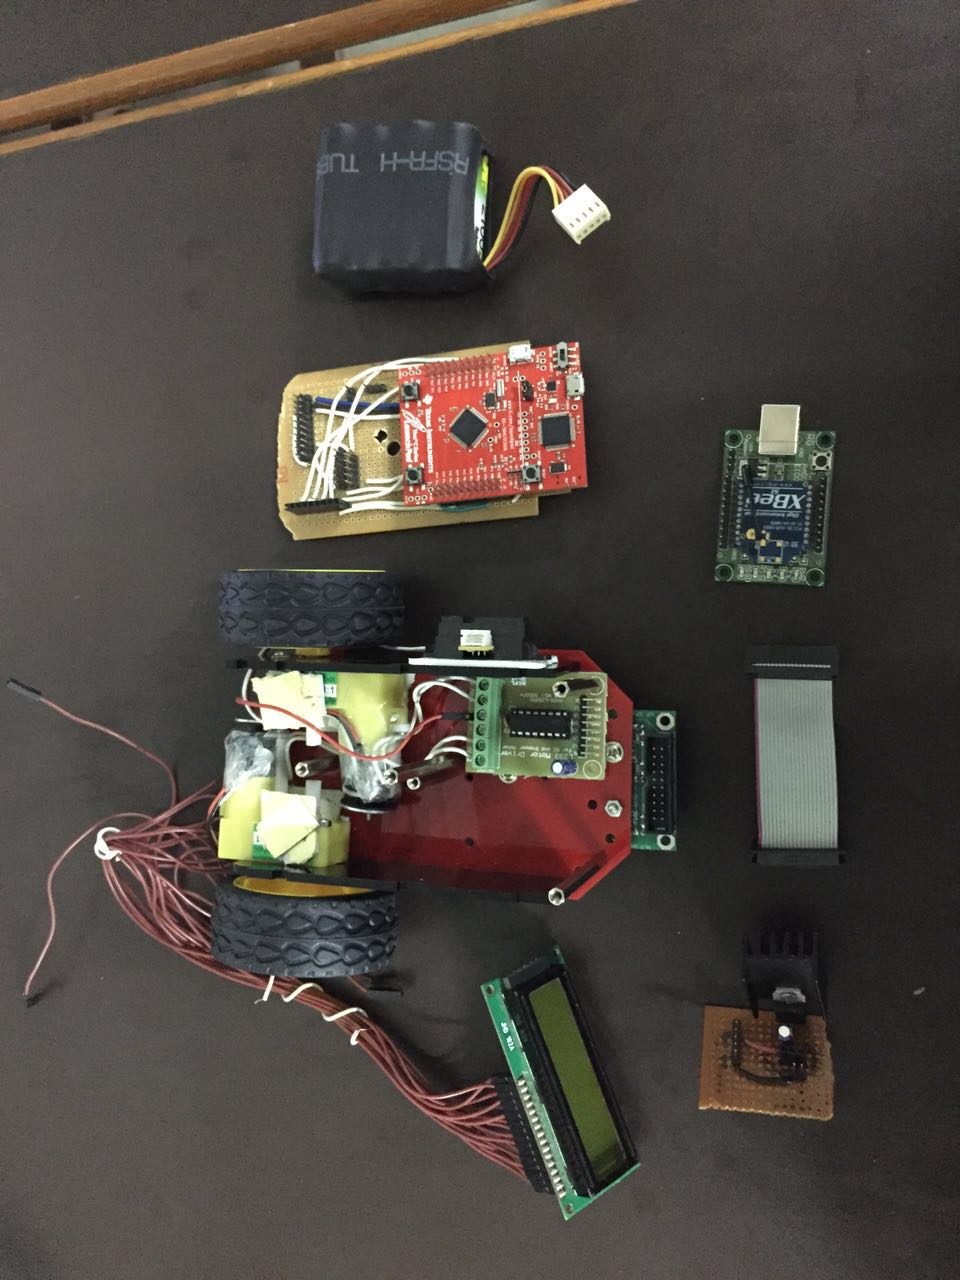
\includegraphics[scale=0.16]{all_components}
		\caption{All the components used to build the Robot.}
	\end{figure}
	\item Assemble the chassis, two DC geared motors and two wheels. Then, connect the motors with the Motor Driver IC.
	\begin{figure}[h]
		\centering
		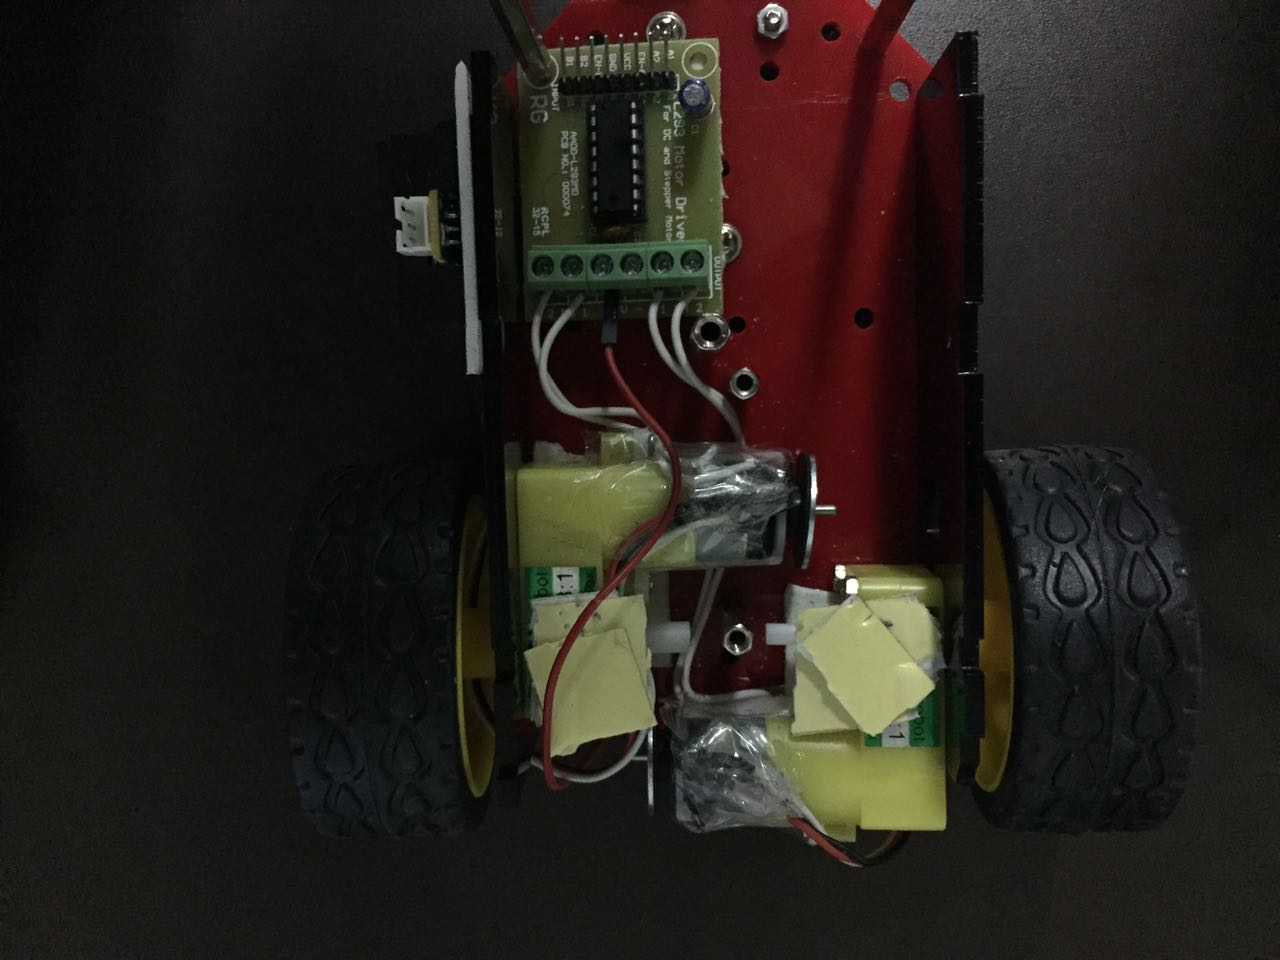
\includegraphics[scale=0.16]{motor_2_ic}
		\caption{Motors and Wheels Attached to Chassis}
	\end{figure}
	\newpage
	\item Connect the White Line Sensors and Caster Wheel to the Chassis.
	\begin{figure}[h]
		\centering
		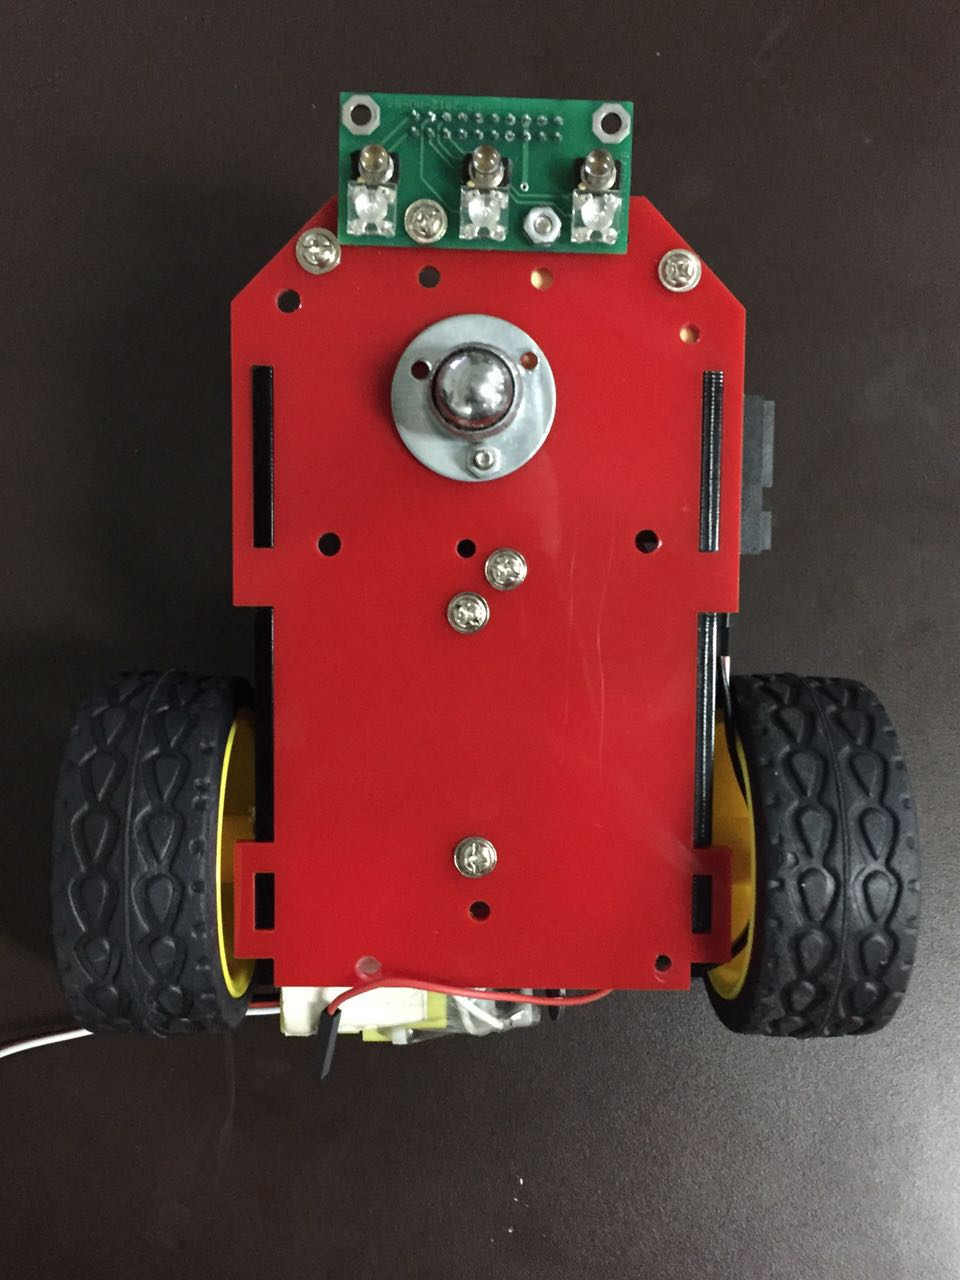
\includegraphics[scale=0.16]{caster_whiteline}
		\caption{Caster Wheel and White Line Sensors Attached to Chassis}
	\end{figure}
	
	\item Attach Sharp Sensor to the Chassis.
	\begin{figure}[h]
		\centering
		\includegraphics[scale=0.16]{a_Sharp}
		\caption{Sharp Sensor Attached to Chassis}
	\end{figure}
	\newpage
	
	\item Attach the Buzzer to the PCB board. Using the male bug strips (4x10) desgin a PCB board to which the Tiva board will be attached.
	\begin{figure}[h]
		\centering
		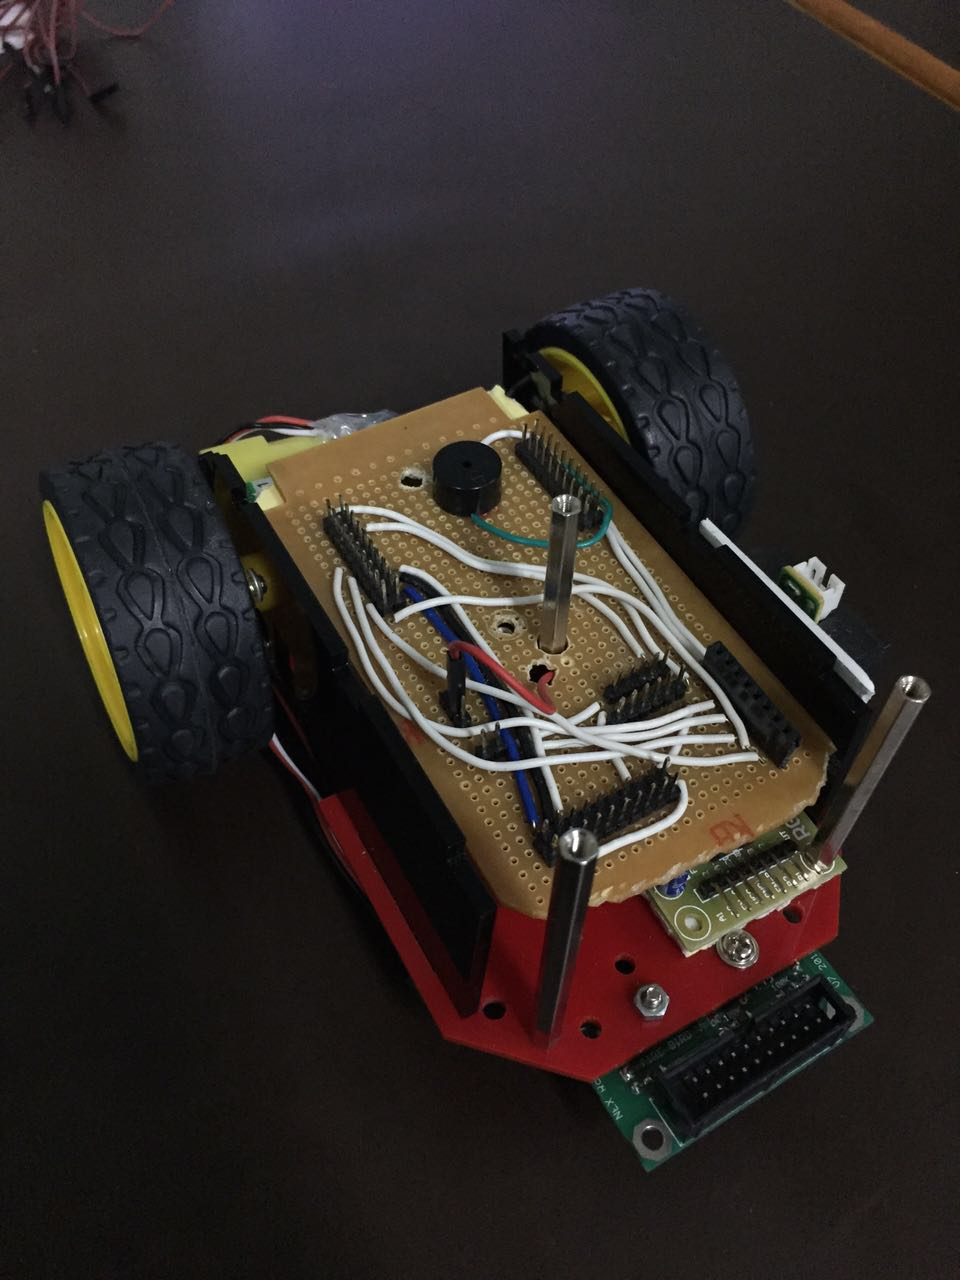
\includegraphics[scale=0.16]{buzzer}
		\caption{Buzzer which would be beneath the Tiva board}
	\end{figure}
	\item Attach Tiva board (TM4C123GXL) on the PCB board.
	\begin{figure}[h]
		\centering
		\includegraphics[scale=0.13]{Tiva_attatched}
		\caption{Tiva Board Fitted}
	\end{figure}
	\newpage
	
	\item Connect White Line Sensors using the 20 pin connector.
	\begin{figure}[h]
		\centering
		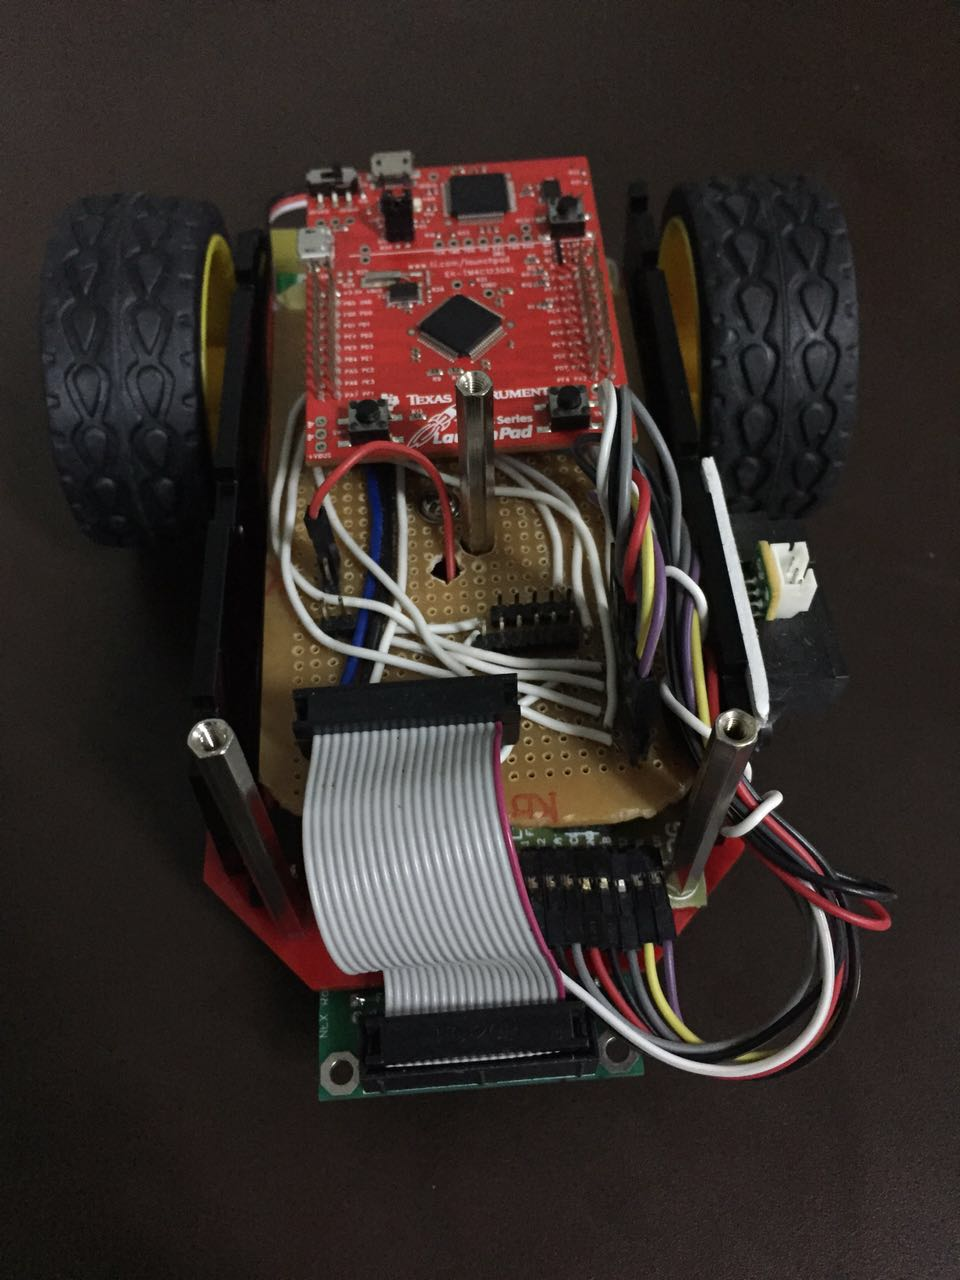
\includegraphics[scale=0.16]{wh_attatched}
		\caption{White Line Sensors are now connected to the Tiva Board.}
	\end{figure}
	
	\item Connect Sharp Sensor and Motor Driver IC to the Tiva Board.
	\begin{figure}[h]
		\centering
		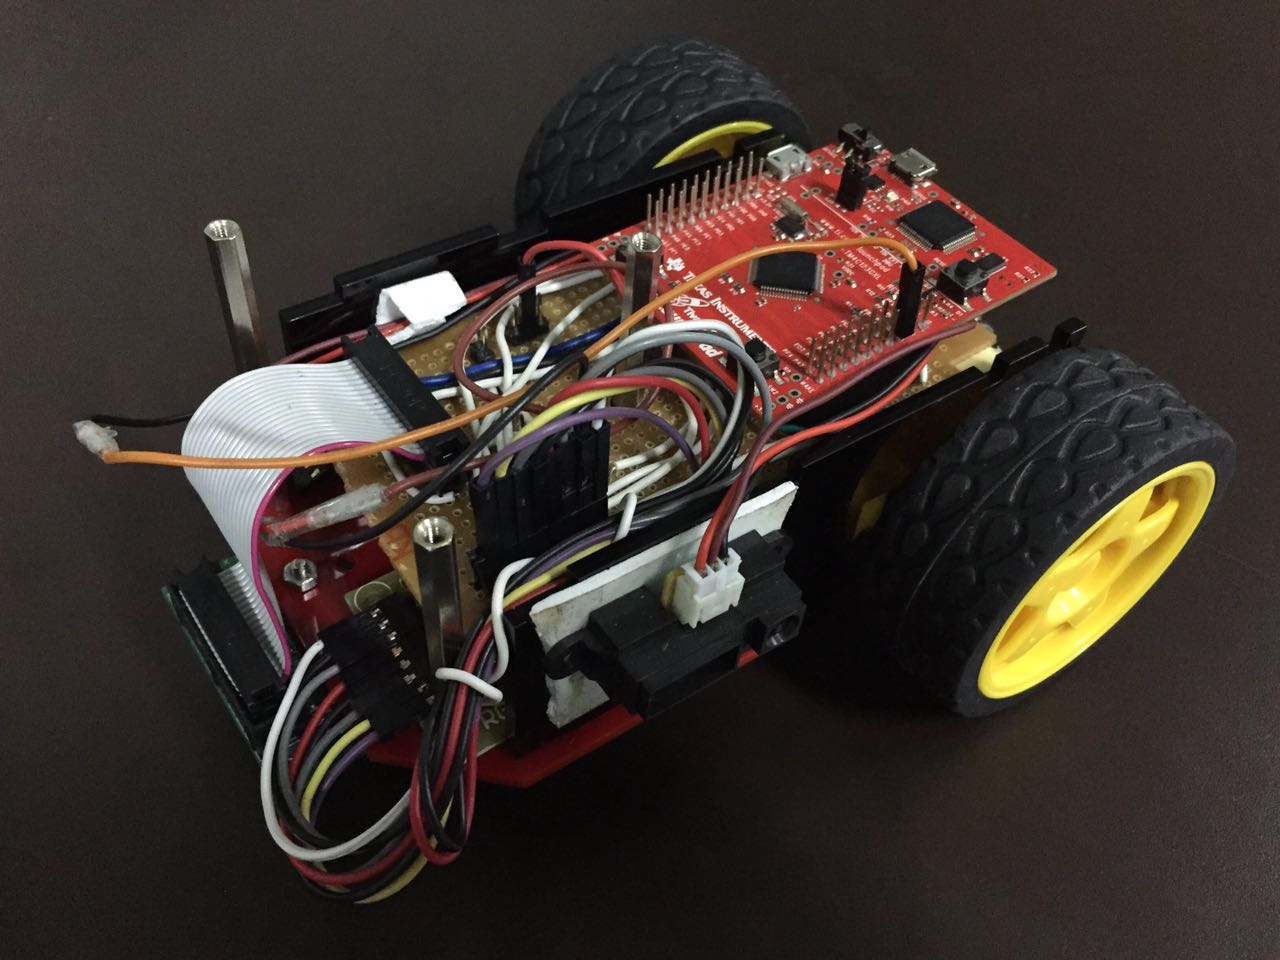
\includegraphics[scale=0.16]{all_connected}
		\caption{Sharp Sensor and Motor Driver IC are now connected to the Tiva Board.}
	\end{figure}
	\newpage
	
	\item Connect the LCD to the Tiva Board.
	\begin{figure}[h]
		\centering
		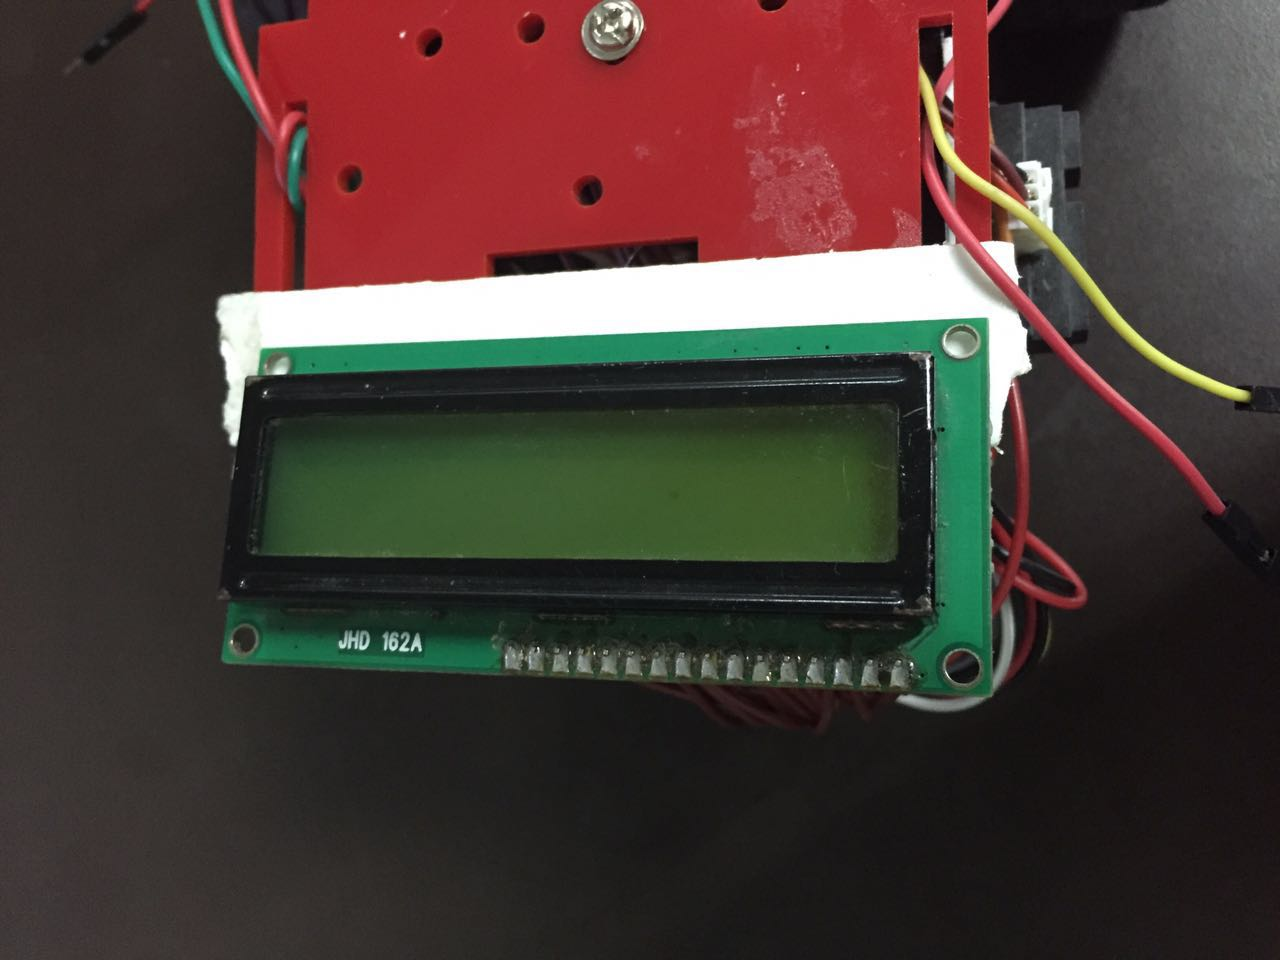
\includegraphics[scale=0.16]{lcd_a}
		\caption{LCD after being attached to the Robot.}
	\end{figure}
	
	\item Connect the XBee to the Tiva Board.
	\begin{figure}[h]
		\centering
		\includegraphics[scale=0.16]{XBee_a}
		\caption{XBee after being attached to the Robot.}
	\end{figure}
	\newpage
	
	\item Connect the Voltage Regulator Circuit and Battery to the Tiva Board.
	\begin{figure}[h]
		\centering
		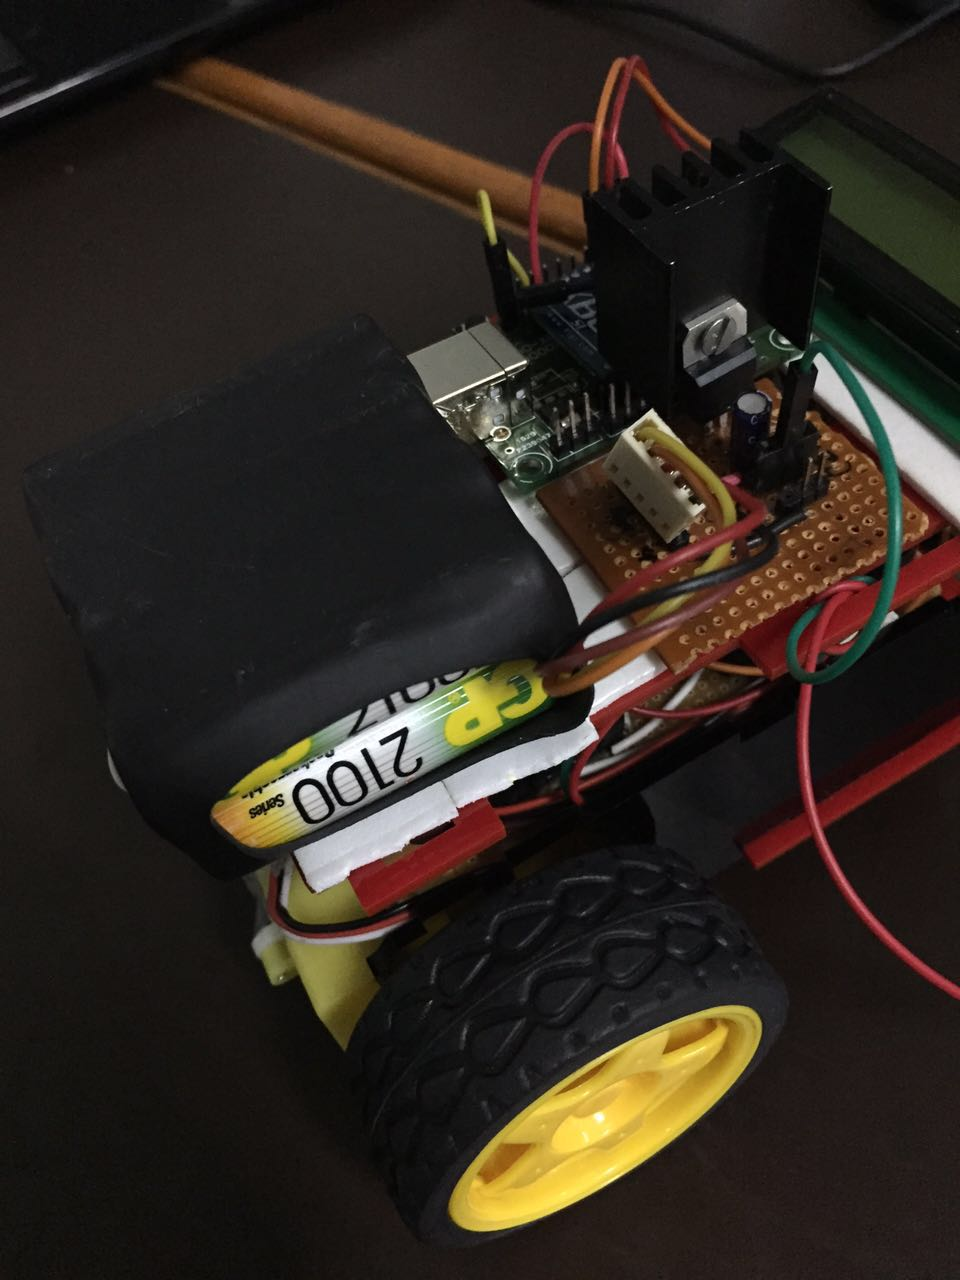
\includegraphics[scale=0.16]{battery_a}
		\caption{ Voltage Regulator Circuit and Battery  after being attached to the Robot}
	\end{figure}

	\item When the LCD is facing up the following photo can be seen to understand how to make the battery connections.
	\begin{figure}[h]
		\centering
		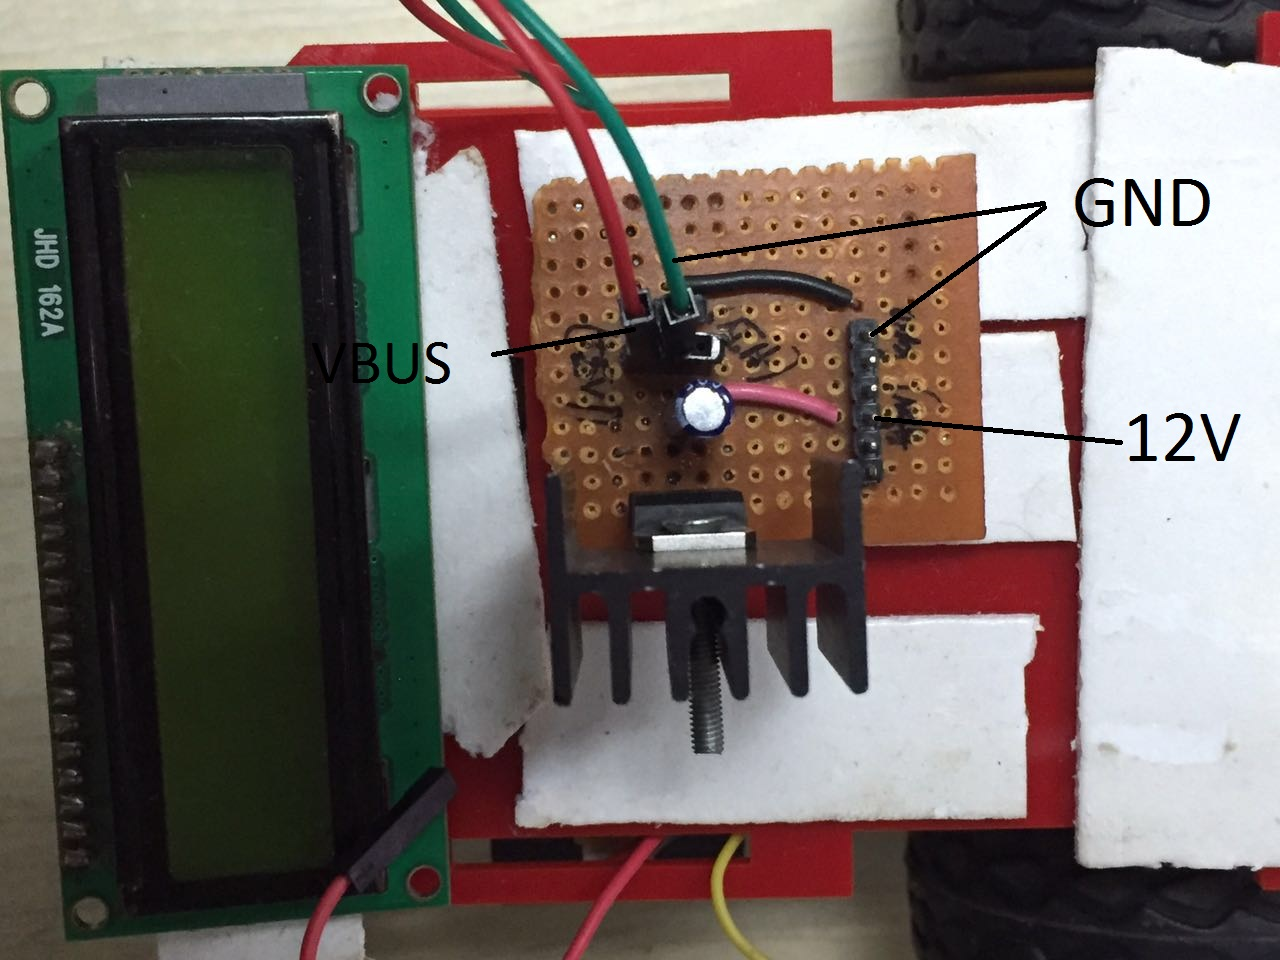
\includegraphics[scale=0.16]{battery_config}
		\caption{ Configuration of battery}
	\end{figure}
	\newpage
	\item Now all the Components are attached to the Robot.
	\begin{figure}[h]
		\centering
		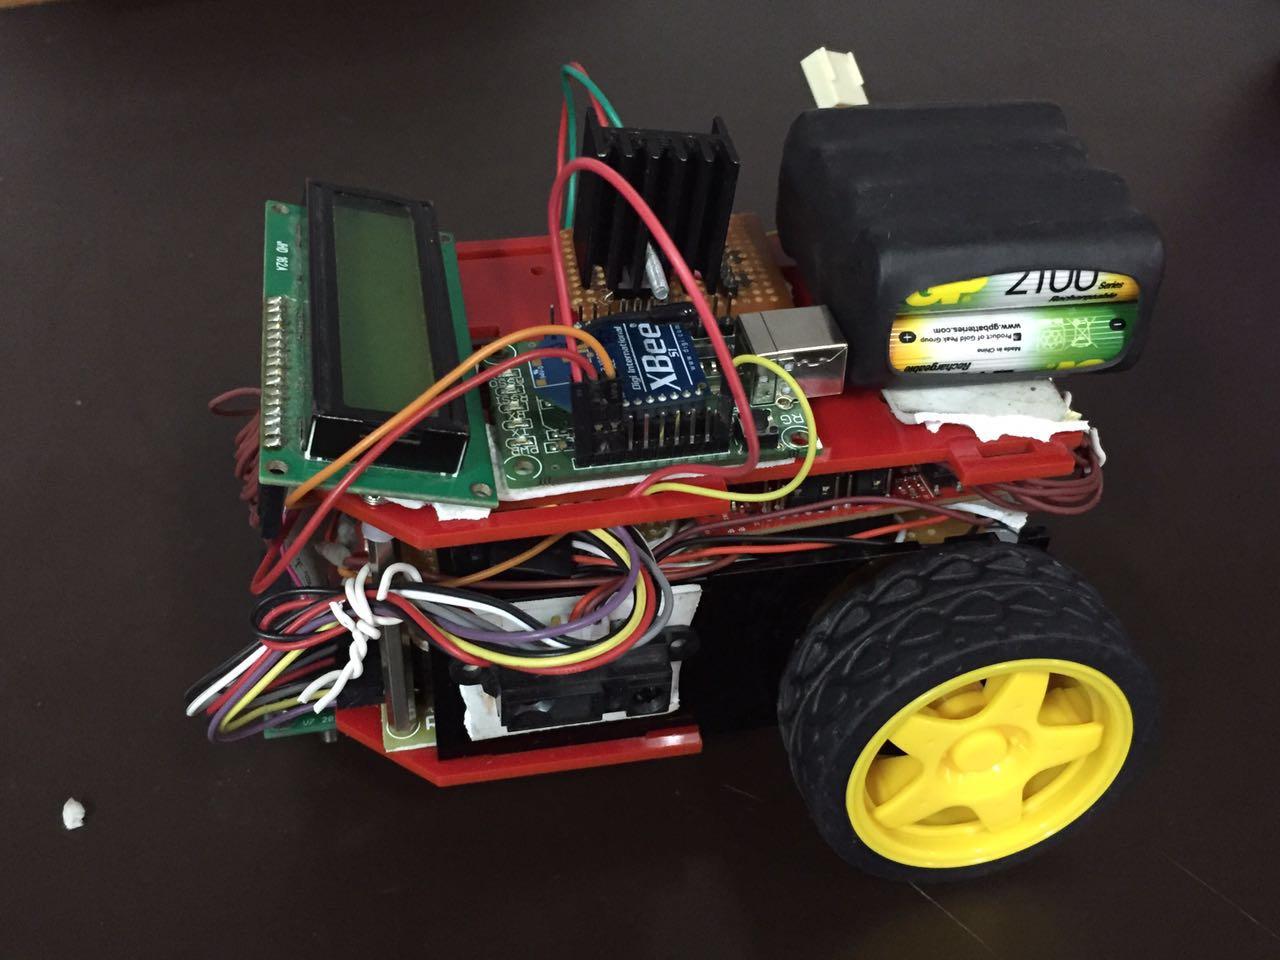
\includegraphics[scale=0.16]{robot}
		\caption{Tiva Robot.}
	\end{figure}
	\newpage
\end{enumerate}

\section{Software and Code}
\begin{itemize}
	\item For programming Tiva board we used \textbf{Code Composer Studio v6.1.3}. It can be downloaded from the link given below.\\
	\href{http://www.ti.com/tool/ccstudio}{Download link}
	\item Tutorials on creating new project in Code Composer Studio and some basic program to configure the port pins of Tiva can be found at \\
	\href{https://www.cse.iitb.ac.in/~erts/html_pages/Resources/Tiva/TM4C123G_LaunchPad_Workshop_Workbook.pdf}{this link}
	\item Code for State Collection on the robot mentioned in this manual is available at the Github repository.
	\href{https://github.com/eYSIP-2016/Robot_State_Collector/tree/master/code/Tiva}{Github link}
\end{itemize}





\end{document}

